\subsection{Incoming alert stream}\label{subsec:alertStream verification}

SCiMMA delivers alerts to Rubin infrastructure through Hopskotch. Hopskotch is a service which provides a publish-subscribe capability for astrophysical alerts. Hopskotch sends a data packet to the Rubin EFD with the following type:

\begin{lstlisting}
        {"namespace": "lsst.scimma",
         "type": "record",
         "name": "ToO_alert",
         "fields": [
               {"name": "alert_type",
                 "type": "string"},
               {"name": "event_trigger_timestamp",
                 "type": "string"},
               {"name": "reward_map",
                 "type": {"type": "array",
                          "items": "boolean"}},
               {"name": "reward_map_nside",
                 "type": "int"},
               {"name": "is_test",
                 "type": "boolean"},
               {"name": "is_update",
                 "type": "boolean"}
                   ]
                }
\end{lstlisting}

The data sent in an alert packet is received at the EFD, where the scheduler CSC collects it. While the Rubin architecture to process incoming alerts has been in place for some time, the receipt of alert data at the EFD from the Rubin ToO group on the SCiMMA Hopskotch service.

\begin{figure}
    \centering
    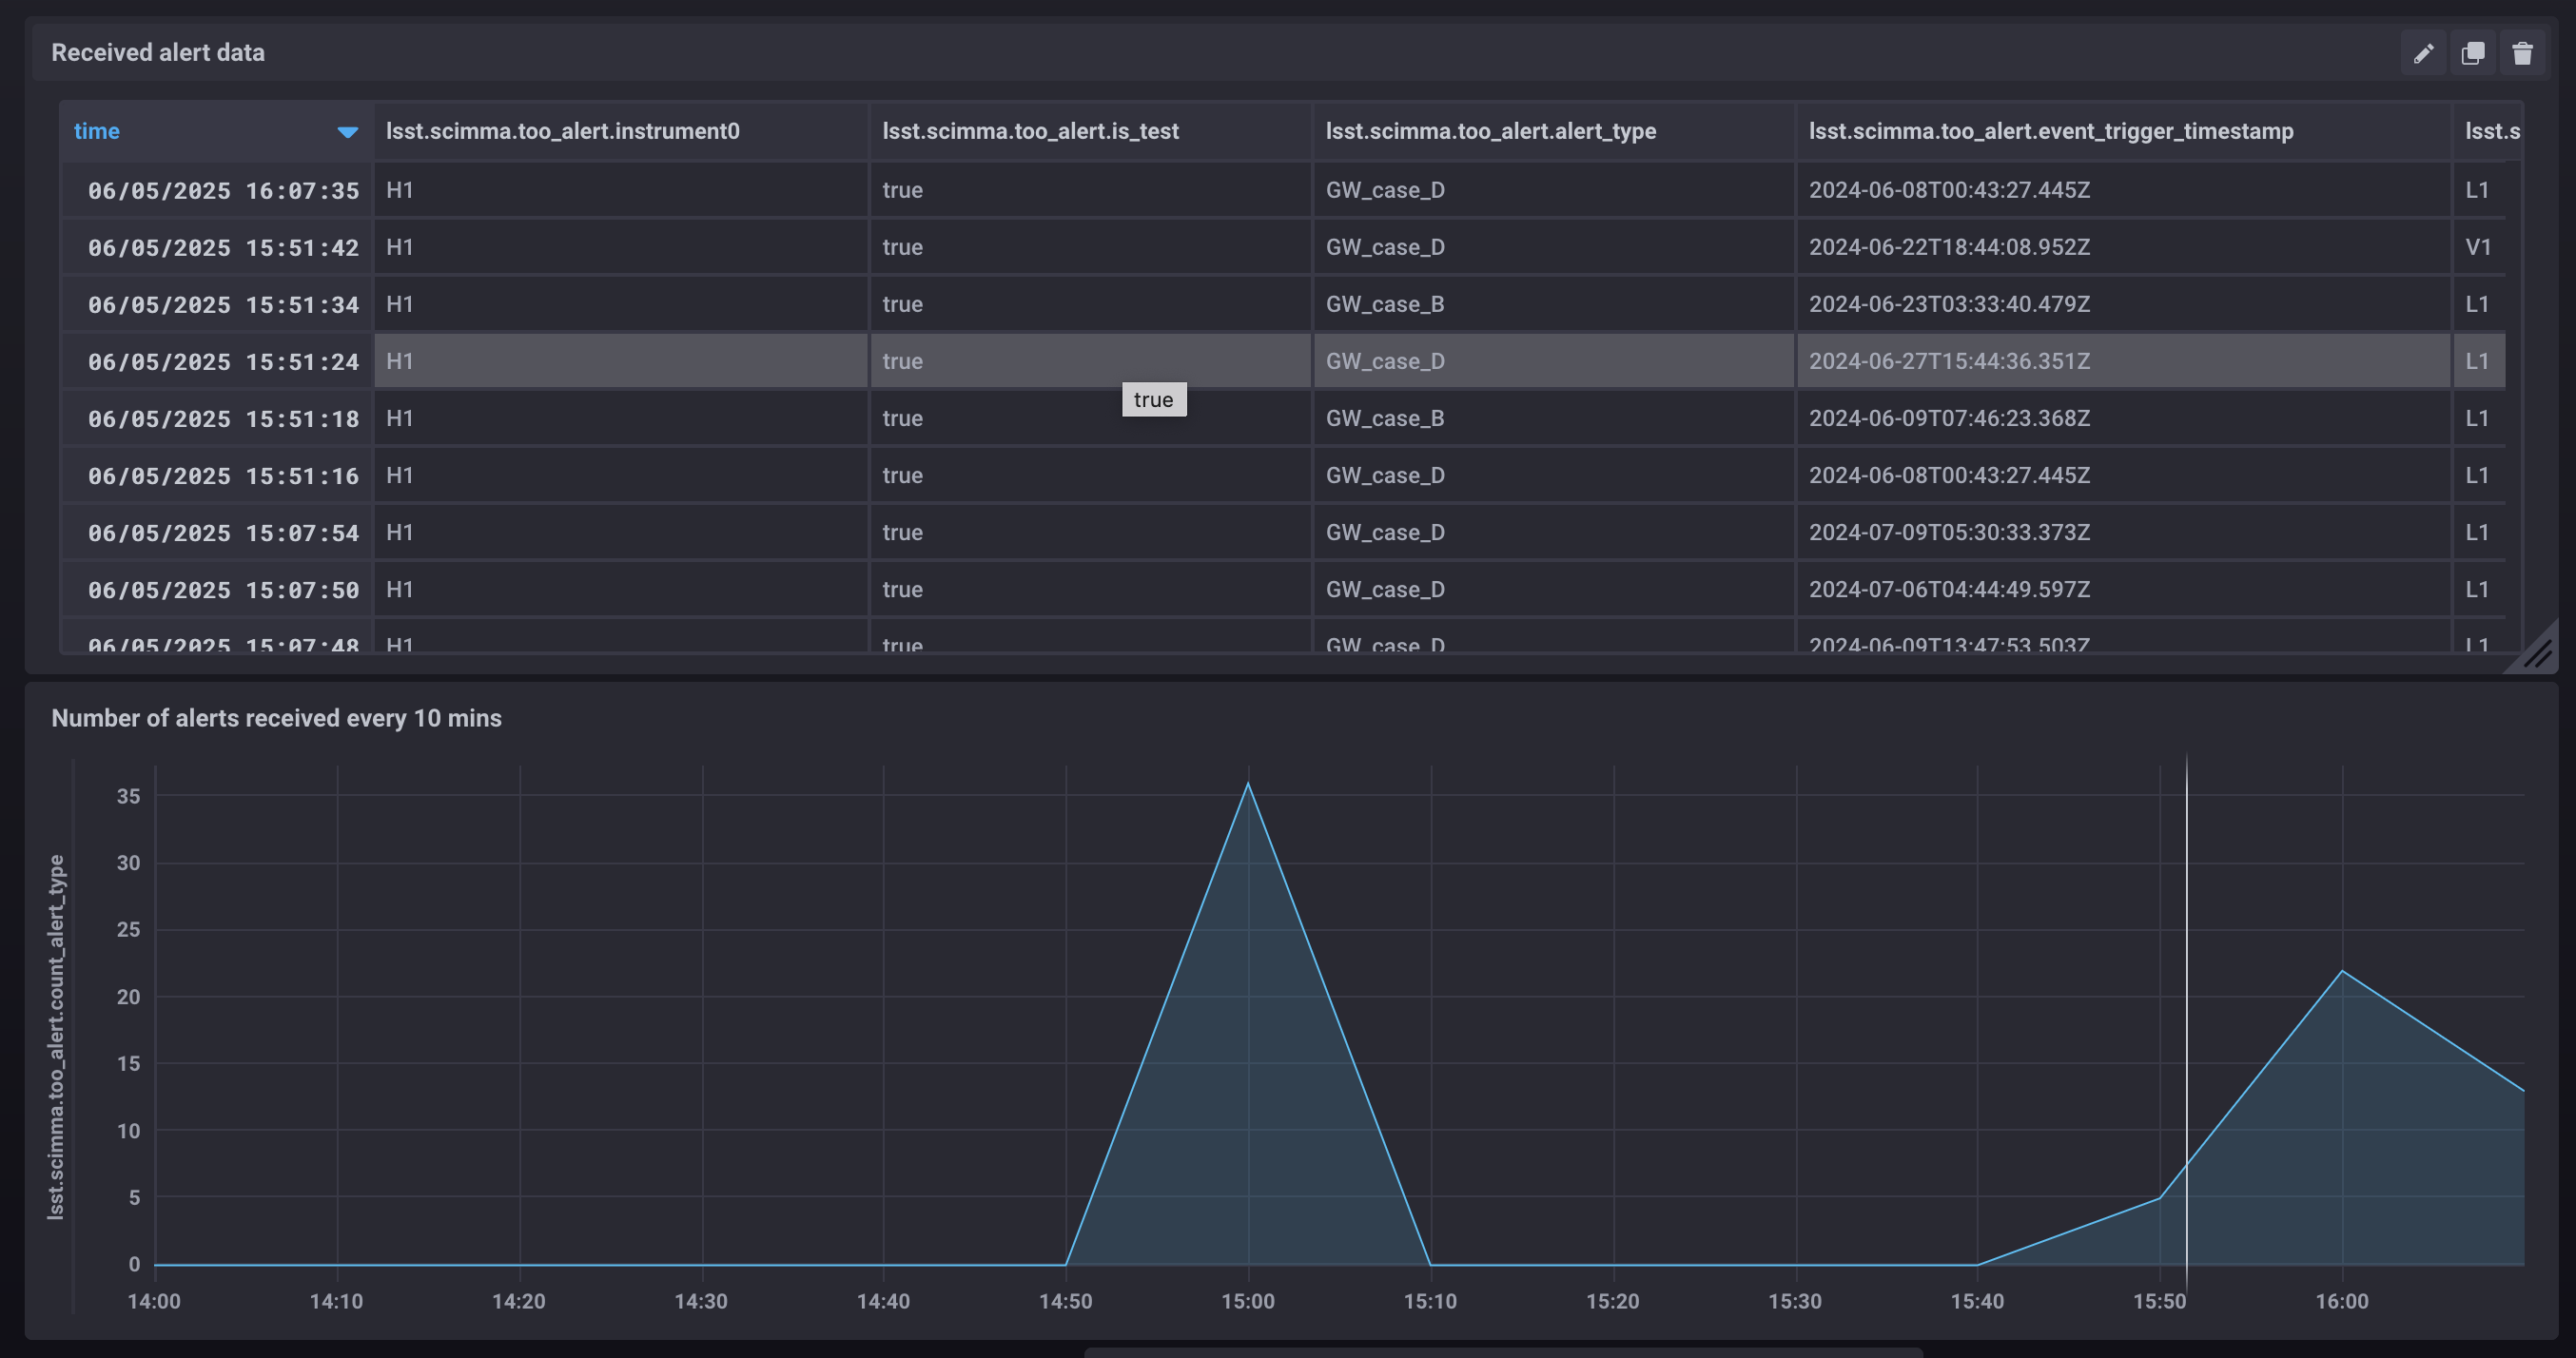
\includegraphics[width=\linewidth]{figures/image.png}
    \caption{The results of the SCiMMA end-end test, demonstrating that alerts are received at EFD from the SCiMMA alert stream.}
    \label{fig:SCiMMA-test result}
\end{figure}

On June 5, 2025, the SCiMMA group demonstrated the capability to send ToO alert packets to the Rubin EFD, including metadata, skymap data, and alert identifiers.

\subsection{The Rubin Scheduler}\label{subsec:Scheduler verification}

The individual alert types have different community defined strategies, as listed in \cite{RubinToO2024}. Early iterations of these strategies have been implemented to the Rubin scheduler, but never tested with skymaps reflective of the alert type. To verify the individual strategy output, we performed tests on simulated ToO's in the Rubin scheduler, using relevant alert, sky, and LSSTCam filter conditions.

To test each ToO strategy, a simulated LSST survey was injected with a ToO of the relevant type and skymap characteristics. The ToO was then handled by the scheduler, which planned and executed the observations following the recommendations from \cite{RubinToO2024}. We summarize the results in \ref{subsubsec:SVRequiredValidation}-\ref{subsubsec:SVOptionalValidation}, and provide the complete results of these simulations in appendix \ref{sec:validationResults}.

\subsubsection{Anticipated ToO strategies during the SV period}\label{subsubsec:SVRequiredValidation}

As recommended by \cite{PSTN-056}, PHA and high-energy neutrino alerts should start as soon as possible. Additionally, given the LVK observing schedule, all GW alerts should start as soon as possible to maximize the overlap of GW alerts and Rubin observations. Therefore, all strategies from table \ref{table:ToOStrategies_sched} except for galactic SN, lensed BNS, and large GW skymaps are considered required for SV.

\begin{table}[]
\centering
\begin{tabular}{|l|l|}
\hline
ToO strategy from ToO 2024 recommendation & Testing result       \\ \hline
GW: NS, gold                              & Pass                 \\ \hline
GW: unidentified source, gold             & Pass                 \\ \hline
GW: NS, silver                            & Pass                 \\ \hline
GW: unidentified source, silver           & Pass                 \\ \hline
GW: BBH, dark time, nearby event                             & Pass, with caveats \\ \hline
GW: BBH, dark time, distant event                              & Pass \\ \hline
GW: BBH, bright time                                & Pass \\ \hline
Neutrino                                  & Pass                 \\ \hline
Potentially hazardous asteroid                      & Pass                 \\ \hline
\end{tabular}
\caption{The results of strategy testing in the Rubin scheduler for SV required strategies.}
\label{tab:SVRequiredStrategy results}
\end{table}

All SV-required ToO strategies passed validation tests in the Rubin scheduler. Minor complications with the BBH, dark time, nearby event strategy were identified during testing. Particularly, the cadence of (1, 3, 8, 10, 40) nights of observation in the ugi filter set is not guaranteed, since the u-band is removed from the camera on a 14-day cadence. There is the possibility that the u band will not be available for all planned nights of observation. Depending on the circumstance, either the cadence of observation should be adjusted, or the filter set should be adjusted to gri, which will always be available in LSSTCam.

\subsubsection{Additional ToO strategies to be pursued during SV}\label{subsubsec:SVOptionalValidation}

While galactic SN, lensed BNS, and large GW skymaps are not expected during the SV surveys due to lower event rates, implementations exist in the Rubin scheduler, and the scientific impact of any of these ToO's is significant. Support for these ToO's remains a priority and events during the SV period should be pursued without reservations, provided the observing strategy is implemented and ready.

\begin{table}[]
\centering
\begin{tabular}{|l|l|}
\hline
ToO strategy from ToO 2024 recommendation & Testing result       \\ \hline
Galactic SN                              & Pass                 \\ \hline
Lensed BNS                              & Pass, with caveats                 \\ \hline
GW: large skymap                              & Not supported                 \\ \hline
\end{tabular}
\caption{The results of strategy testing in the Rubin scheduler for additional ToO strategies.}
\label{tab:SVOptionalStrategy results}
\end{table}

The galactic SN strategy passed validation tests. Discussions about using a different scheduler configuration for the case of a galactic SN are ongoing, and additional testing may be required to evaluate this option. The lensed BNS strategy passed, with some caveats about epoch timing. Epoch timing is affected significantly by set/rise time, since the requested number of observations on a given night in either the large or small sky-area case is near a complete night. The priorities of inaccurate epoch timing or fewer visits is currently being discussed with the Rubin science community. For large GW skymaps, coverage should be coordinated with the SCOC, and the Rubin scheduler will not support these kinds of alerts.

\subsection{Full system tests}\label{subsec:systemTests verification}

The previous verifications in sections \ref{subsec:alertStream verification} - \ref{subsec:Scheduler verification} were needed to validate individual components of the ToO workflow from figure \ref{fig:workflowDiagram}. With the previous components validated in isolation, it is imperative to test the system in its entirety. To do so, we injected a mock ToO event in a previously imaged region, and considered the case where template images either exist or do not exist. Considering both of these cases covers the complete parameter space of PP conditions, with a non-templated region being the more likely possibility during SV.

For both cases, we consider observations of the same region of the sky where templates exist. In the non-templated test case, we ignore existing templates to provide a 1:1 comparison to the typical PP workflow.

\subsubsection{Non-templated region}\label{subsubsec:systemTests NonTemplated}


\subsubsection{Templated region}\label{subsubsec:systemTests templated}
